% !TEX TS-program = pdflatex
% !TEX encoding = UTF-8 Unicode
% 
% This file is a template using the "beamer" package to create slides for a talk or presentation
% - Talk at a conference/colloquium.
% - Talk length is about 20min.
% - Style is ornate.
% 
% MODIFIED by Jonathan Kew, 2008-07-06
% The header comments and encoding in this file were modified for inclusion with TeXworks.
% The content is otherwise unchanged from the original distributed with the beamer package.
\documentclass{beamer}
\usepackage[utf8]{inputenc} % set input encoding (not needed with XeLaTeX)

%%% Examples of Article customizations
% These packages are optional, depending whether you want the features they provide.
% See the LaTeX Companion or other references for full information.

%%% PAGE DIMENSIONS
\usepackage{geometry} % to change the page dimensions
\geometry{a4paper} % or letterpaper (US) or a5paper or....
% \geometry{margin=2in} % for example, change the margins to 2 inches all round
% \geometry{landscape} % set up the page for landscape
%   read geometry.pdf for detailed page layout information

\usepackage{graphicx} % support the \includegraphics command and options

% \usepackage[parfill]{parskip} % Activate to begin paragraphs with an empty line rather than an indent

%%% PACKAGES
\usepackage{booktabs} % for much better looking tables
\usepackage{array} % for better arrays (eg matrices) in maths
\usepackage{paralist} % very flexible & customisable lists (eg. enumerate/itemize, etc.)
\usepackage{verbatim} % adds environment for commenting out blocks of text & for better verbatim
\usepackage{subfig} % make it possible to include more than one captioned figure/table in a single float
% These packages are all incorporated in the memoir class to one degree or another...

%%% HEADERS & FOOTERS
\usepackage{fancyhdr} % This should be set AFTER setting up the page geometry
\pagestyle{fancy} % options: empty , plain , fancy
\renewcommand{\headrulewidth}{0pt} % customise the layout...
\lhead{}\chead{}\rhead{}
\lfoot{}\cfoot{\thepage}\rfoot{}

%%% SECTION TITLE APPEARANCE
\usepackage{sectsty}
\allsectionsfont{\sffamily\mdseries\upshape} % (See the fntguide.pdf for font help)
% (This matches ConTeXt defaults)

%%% ToC (table of contents) APPEARANCE
\usepackage[nottoc,notlof,notlot]{tocbibind} % Put the bibliography in the ToC
\usepackage[titles,subfigure]{tocloft} % Alter the style of the Table of Contents
\renewcommand{\cftsecfont}{\rmfamily\mdseries\upshape}
\renewcommand{\cftsecpagefont}{\rmfamily\mdseries\upshape} % No bold!

%%% END Article customizations
\usepackage{xcolor}
\usepackage{tcolorbox}
\usepackage{lipsum}  % 示例文本
\usepackage{mdframed}
\usepackage{pdfpages}


% R code support
\usepackage{listings}
% \lstset{language=R,  % 设置语言为R
%         basicstyle=\ttfamily, % 设置字体样式
%         numbers=left,  % 行号显示在左侧
%         numberstyle=\small\color{blue},  % 行号样式
%         frame=single,  % 设置代码块的边框
%         backgroundcolor=\color{lightgray},  % 设置代码块的背景颜色
%         }

\usepackage{graphicx}
\usepackage{float}
\usepackage{amsmath}





% 设置R语言代码高亮
\lstdefinestyle{rstyle}{
  language=R,
  basicstyle=\ttfamily,
  numbers=left,
  numberstyle=\tiny\color{gray},
  commentstyle=\color{green!40!black},
  keywordstyle=\color{blue},
  stringstyle=\color{purple},
  morekeywords={read.csv},
  frame=single,
  breaklines=true
}
% 
\title[] % (optional, use only with long paper titles)
{Introduction to Math for DS Group Project}

\subtitle
{Predicting the Premier League Winner}

\author % (optional, use only with lots of authors)
{IMDS Group 24}
% - Give the names in the same order as the appear in the paper.
% - Use the \inst{?} command only if the authors have different
%   affiliation.

\institute[Data Science] % (optional, but mostly needed)
{
  Zehao Qian, Mohammad Jamshaid Iqbal, Chloe Mendez \\ \ \\
  Department of Natural Sciences \\
  Durham University, England, UK
}
% - Use the \inst command only if there are several affiliations.
% - Keep it simple, no one is interested in your street address.

% \date[CFP 2003] % (optional, should be abbreviation of conference name)
% {Conference on Fabulous Presentations, 2003}
% - Either use conference name or its abbreviation.
% - Not really informative to the audience, more for people (including
%   yourself) who are reading the slides online
% \subject{Theoretical Computer Science}
% This is only inserted into the PDF information catalog. Can be left
% out. 
% If you have a file called "university-logo-filename.xxx", where xxx
% is a graphic format that can be processed by latex or pdflatex,
% resp., then you can add a logo as follows:
% \pgfdeclareimage[height=0.5cm]{university-logo}{university-logo-filename}
% \logo{\pgfuseimage{university-logo}}
% Delete this, if you do not want the table of contents to pop up at
% the beginning of each subsection:
\AtBeginSubsection[]
{
  \begin{frame}<beamer>{Outline}
    \tableofcontents[currentsection,currentsubsection]
  \end{frame}
}
% 
% If you wish to uncover everything in a step-wise fashion, uncomment
% the following command: 
%\beamerdefaultoverlayspecification{<+->}
\begin{document}
% 
\begin{frame}
  \titlepage
\end{frame}
% \input{CV.tex}
% 
\begin{frame}
  \tableofcontents
  % You might wish to add the option [pausesections]
\end{frame}
% 
% 
% Structuring a talk is a difficult task and the following structure
% may not be suitable. Here are some rules that apply for this
% solution: 
% 
% - Exactly two or three sections (other than the summary).
% - At *most* three subsections per section.
% - Talk about 30s to 2min per frame. So there should be between about
%   15 and 30 frames, all told.
% 
% - A conference audience is likely to know very little of what you
%   are going to talk about. So *simplify*!
% - In a 20min talk, getting the main ideas across is hard
%   enough. Leave out details, even if it means being less precise than
%   you think necessary.
% - If you omit details that are vital to the proof/implementation,
%   just say so once. Everybody will be happy with that.
% 
% 
\section{Introduction}
\subsection{Intro to Data Set and its Context}
% 
% 
% 
% 
% 
% 
\begin{frame}
  \frametitle{What is Happiness?}
  \begin{figure}
    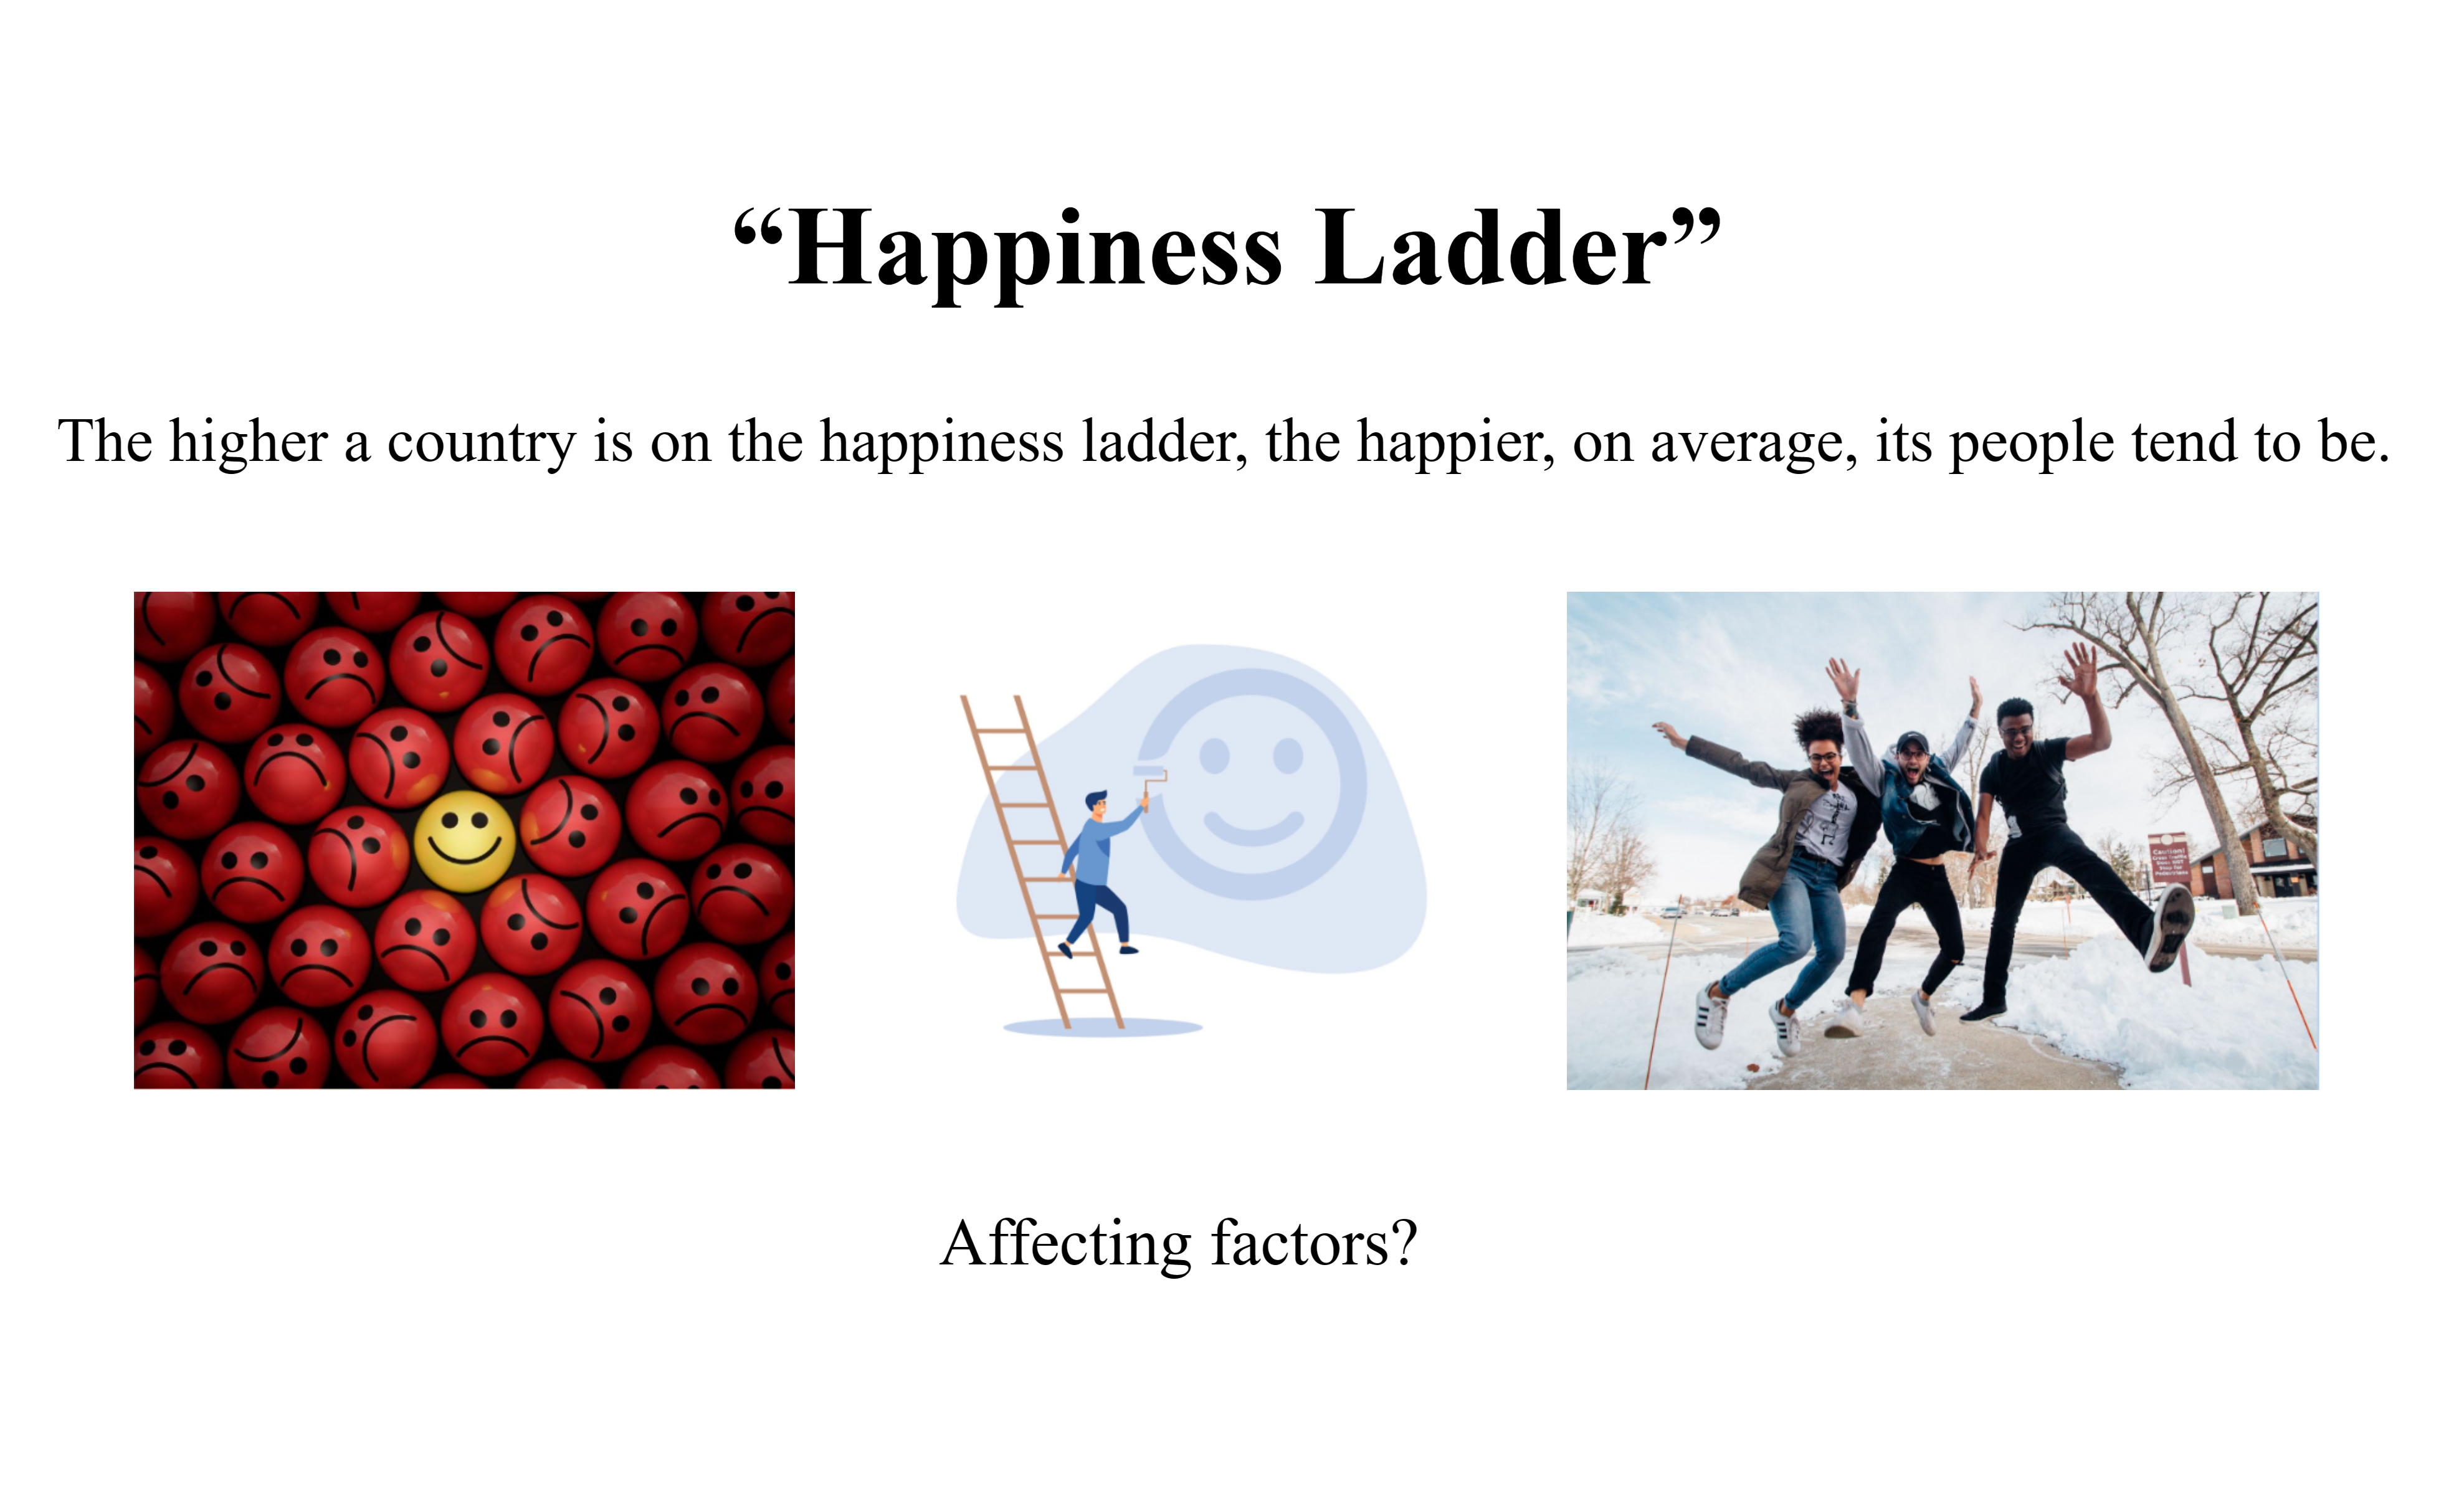
\includegraphics[width=\textwidth]{img/What is happyness.png}
  \end{figure}
\end{frame}
% 
% 
% 
% 
\begin{frame}
  \frametitle{Data Set and its Context}
  \begin{figure}
    
\includegraphics[width=\textwidth]{img/Intro to Dataset.png}
  \end{figure}
\end{frame}
% 
% 
% 
% 
% 
% 
% 
% 
% 
% 
% 
% 
\section{Statistical Modeling}
% 
% 
% 
% 
\subsection{Model Explanation}
% 
% 
% 
% 
\begin{frame}
  \frametitle{Multiple Linear Regression Model}
  \begin{itemize}
    \item \textbf{Model Target:} Some socio-economic indexes are used to predict Ladder Score to assist government decision-making.
    \item \textbf{Independent Variables:} LGDP, Support, HLE, Freedom, Corruption, Continent
    \item \textbf{Dependent Variables:} Ladder Score
    \item \textbf{Model Function:} $input(LGDP, Support,...) \Rightarrow output(Ladder\ Score)$
          $ Ladder Score = \beta_0 + \beta_1 * LGDP + \beta_2 * Support + ... + \epsilon $
    \item \textbf{Optimization Target:} Making the model with the \textcolor{red}{best subset} and \textcolor{red}{higher Adjusted R-squared}. $
            \left\{
            \begin{matrix}
              Select\ the\ independent\ variables \\
              Update\ \beta\ and\ \epsilon\ to\ minimize\ the\ residual\ sum\ of\ squared
            \end{matrix}
            \right.
          $
  \end{itemize}
  % 
  % 
  % 
  % 
\end{frame}
% 
% 
% 
% 
% \begin{frame}{Comparison of Linear Regression Models}
\begin{frame}{Why we choose Multiple Linear Regression Model}
  \begin{figure}
    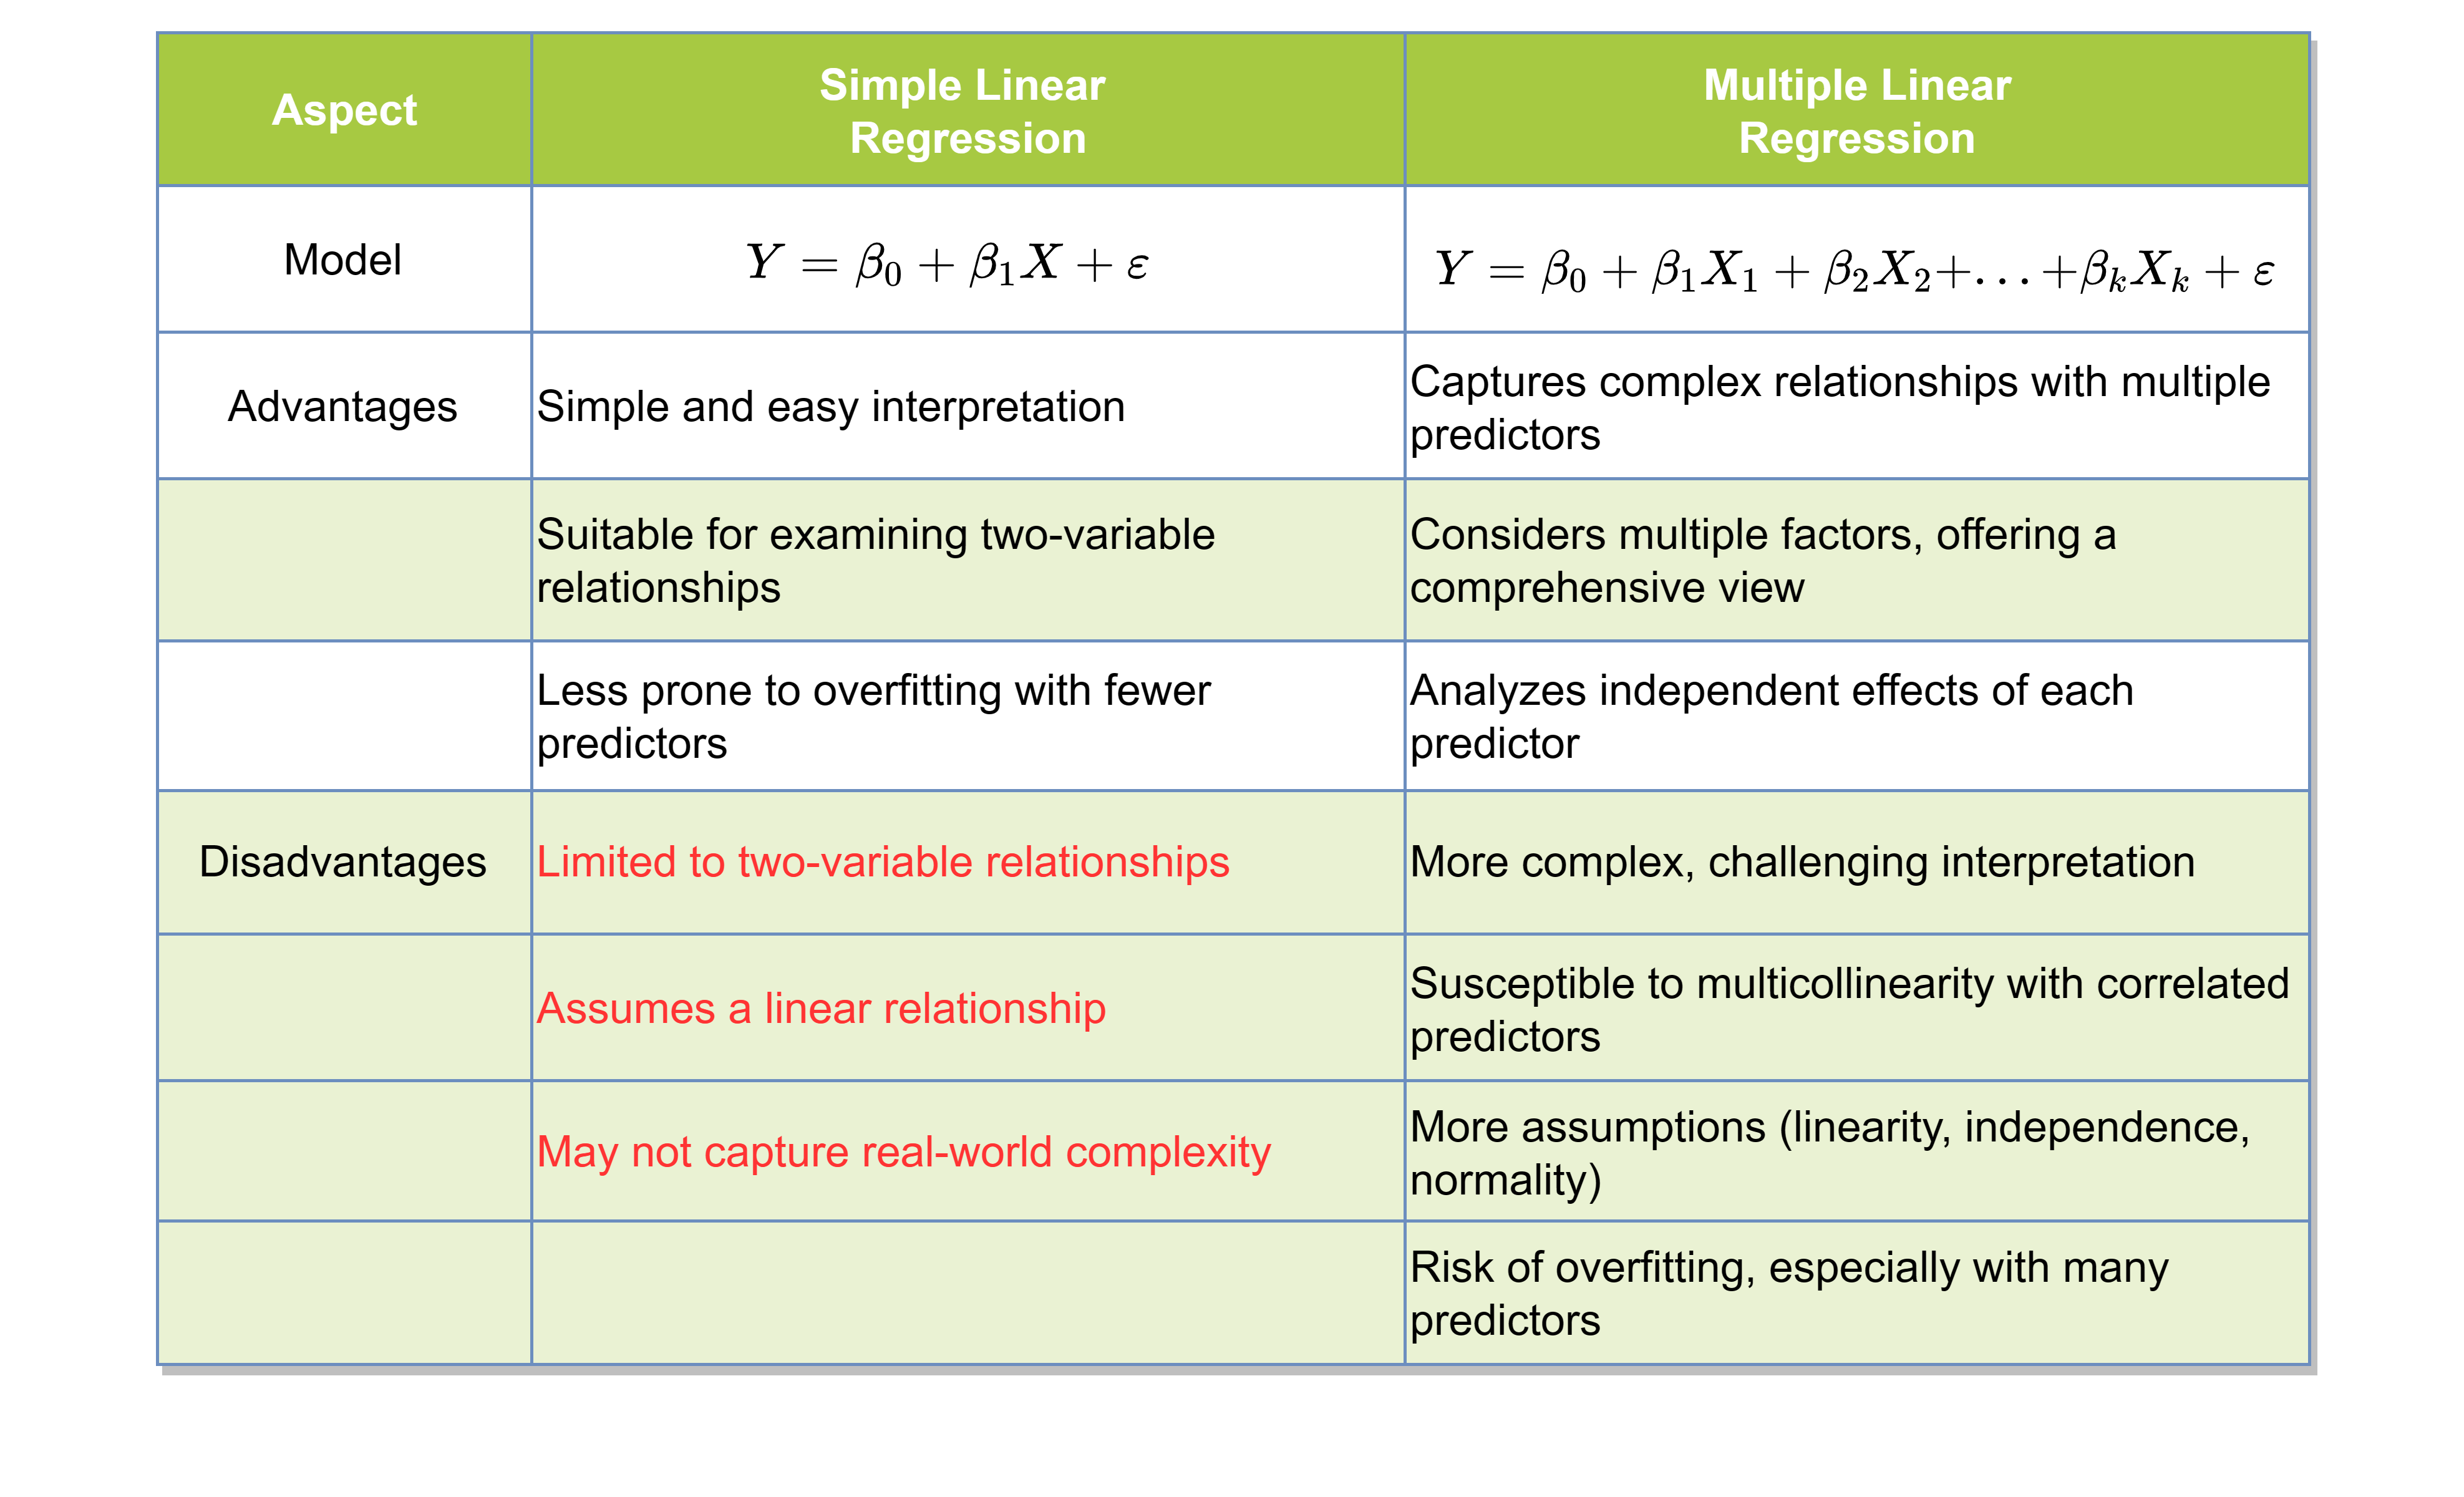
\includegraphics[width=\textwidth]{img/Why choose this model.png}
  \end{figure}
\end{frame}
% 
% 
% 
% 
\subsection{Model Construction}
% 
% 
% 
% 
\begin{frame}
  \frametitle{Constructing the Model -- Data Processing}
  \begin{figure}
    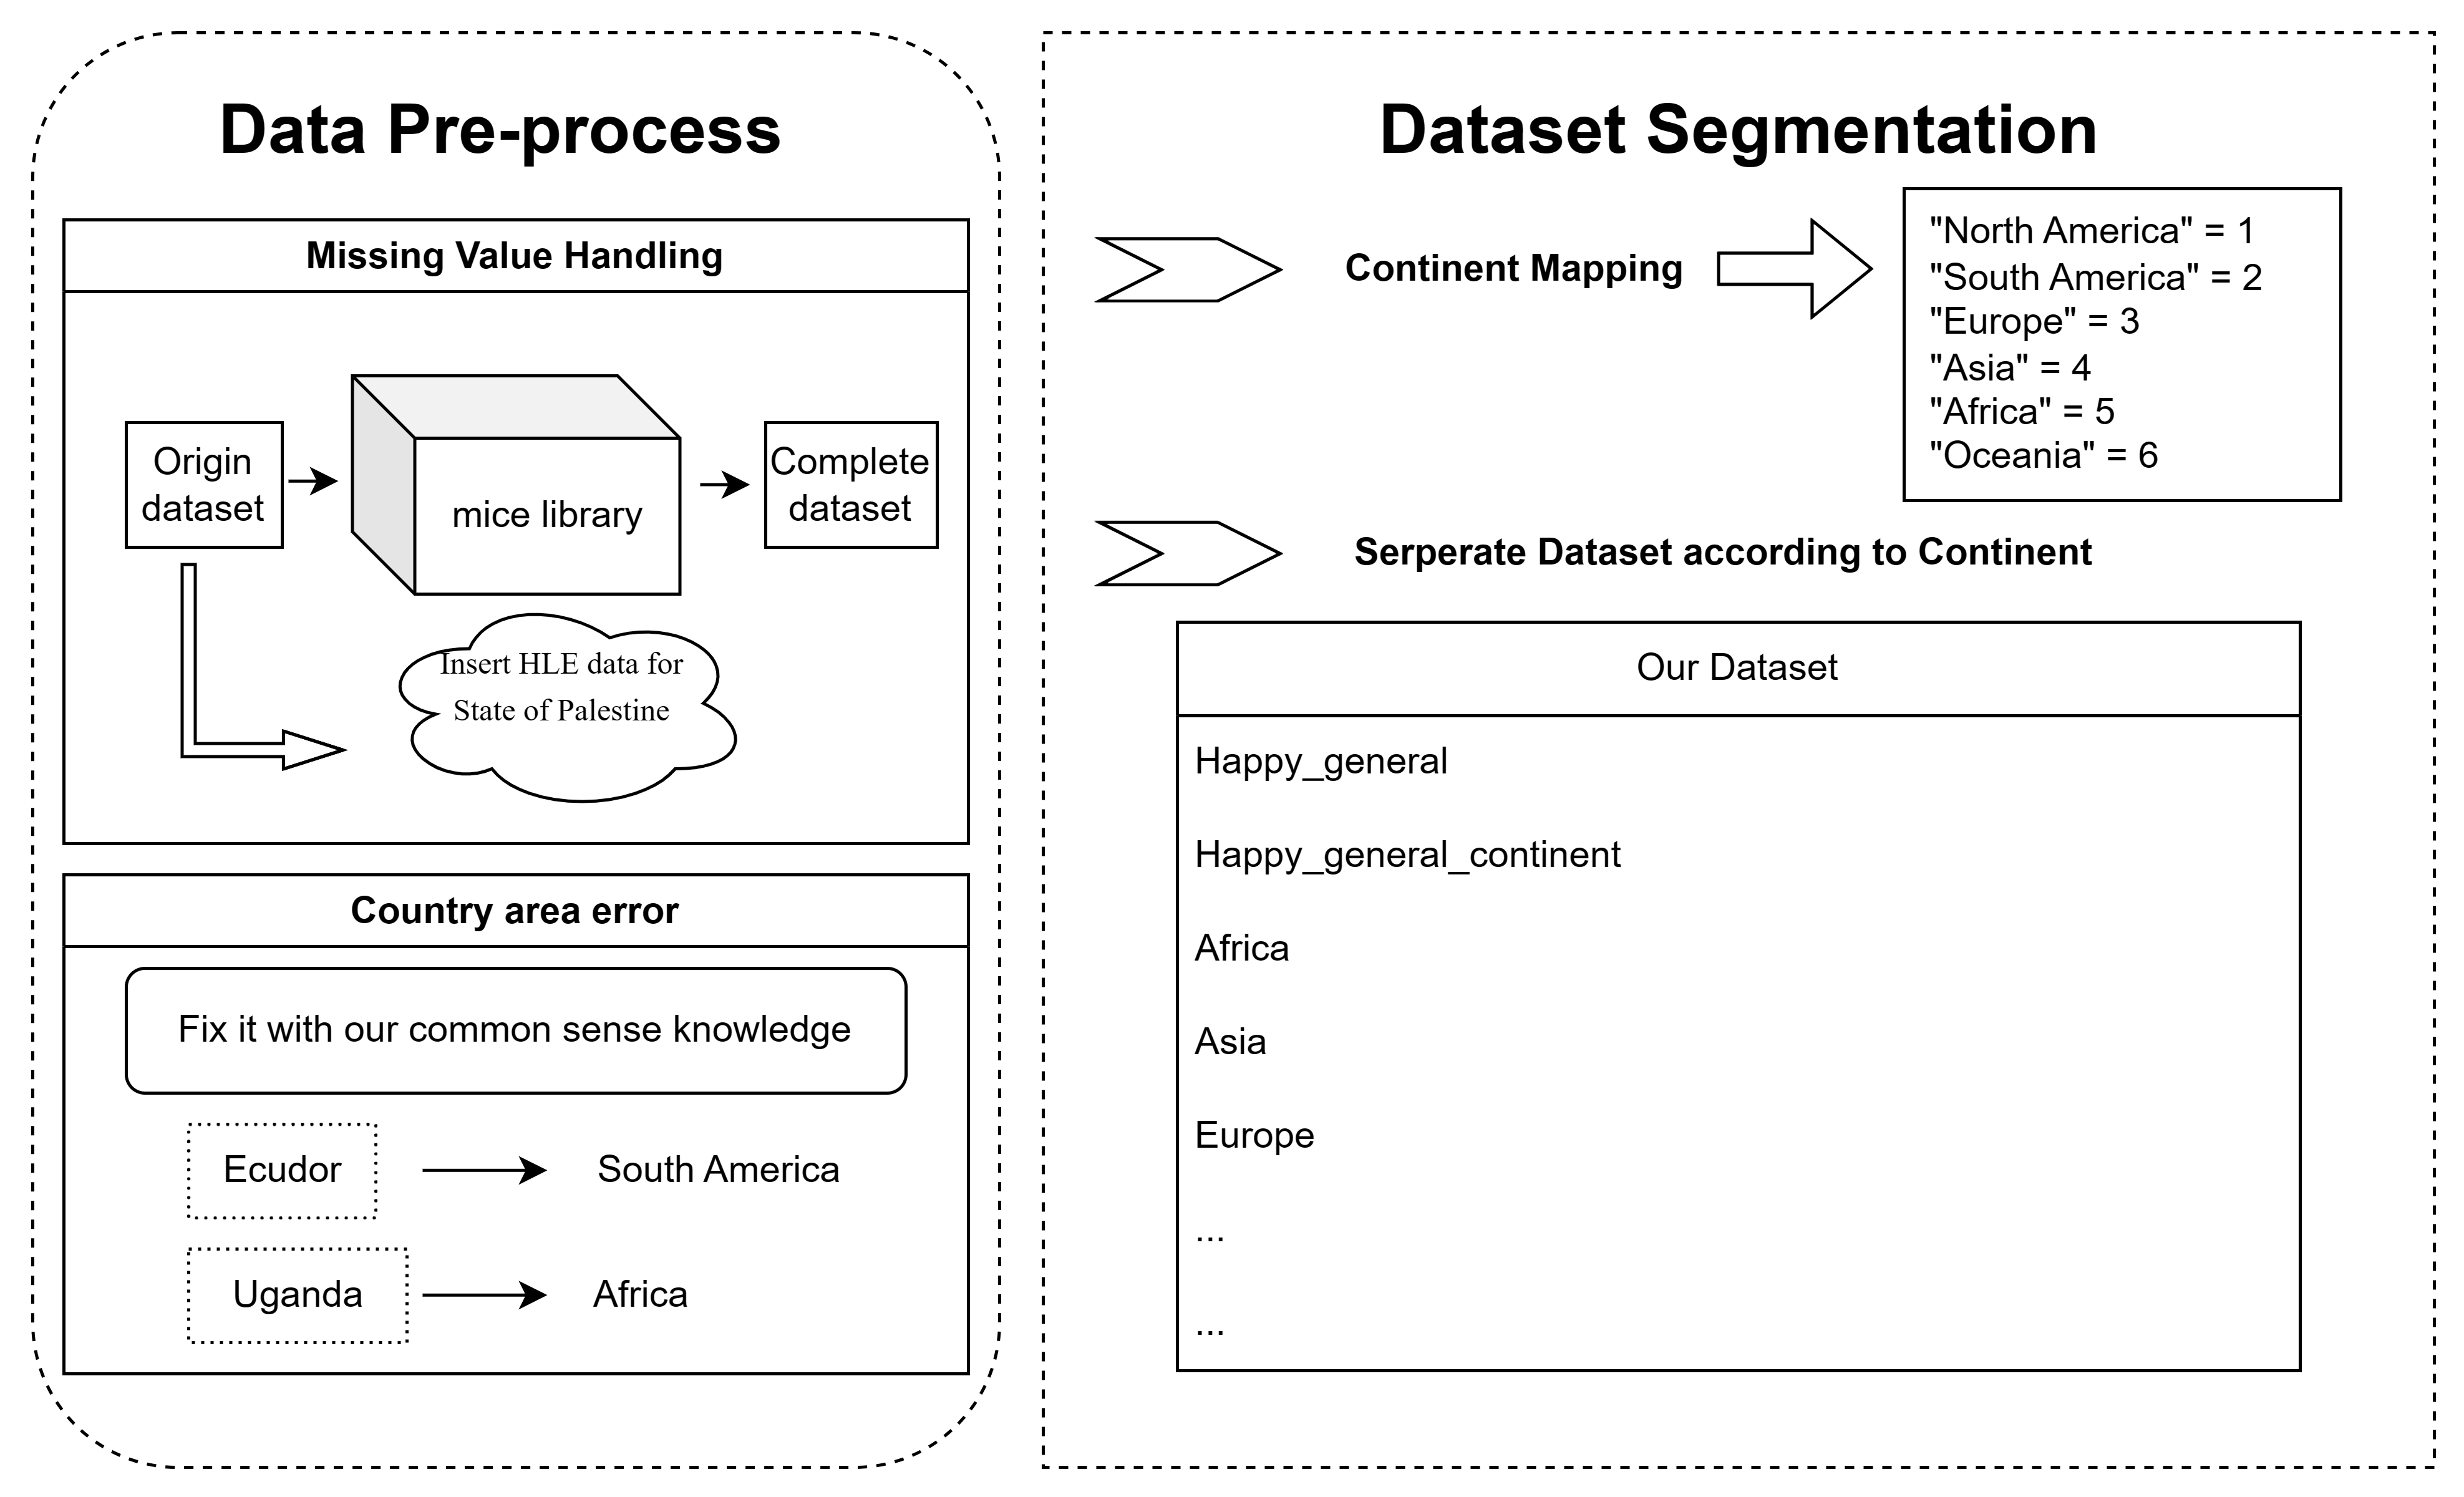
\includegraphics[width=\textwidth]{img/Data Process.png}
  \end{figure}
\end{frame}
% 
% 
% 
% 
\begin{frame}
  \frametitle{Constructing the Model -- Dataset Inspectation}
  \begin{figure}
    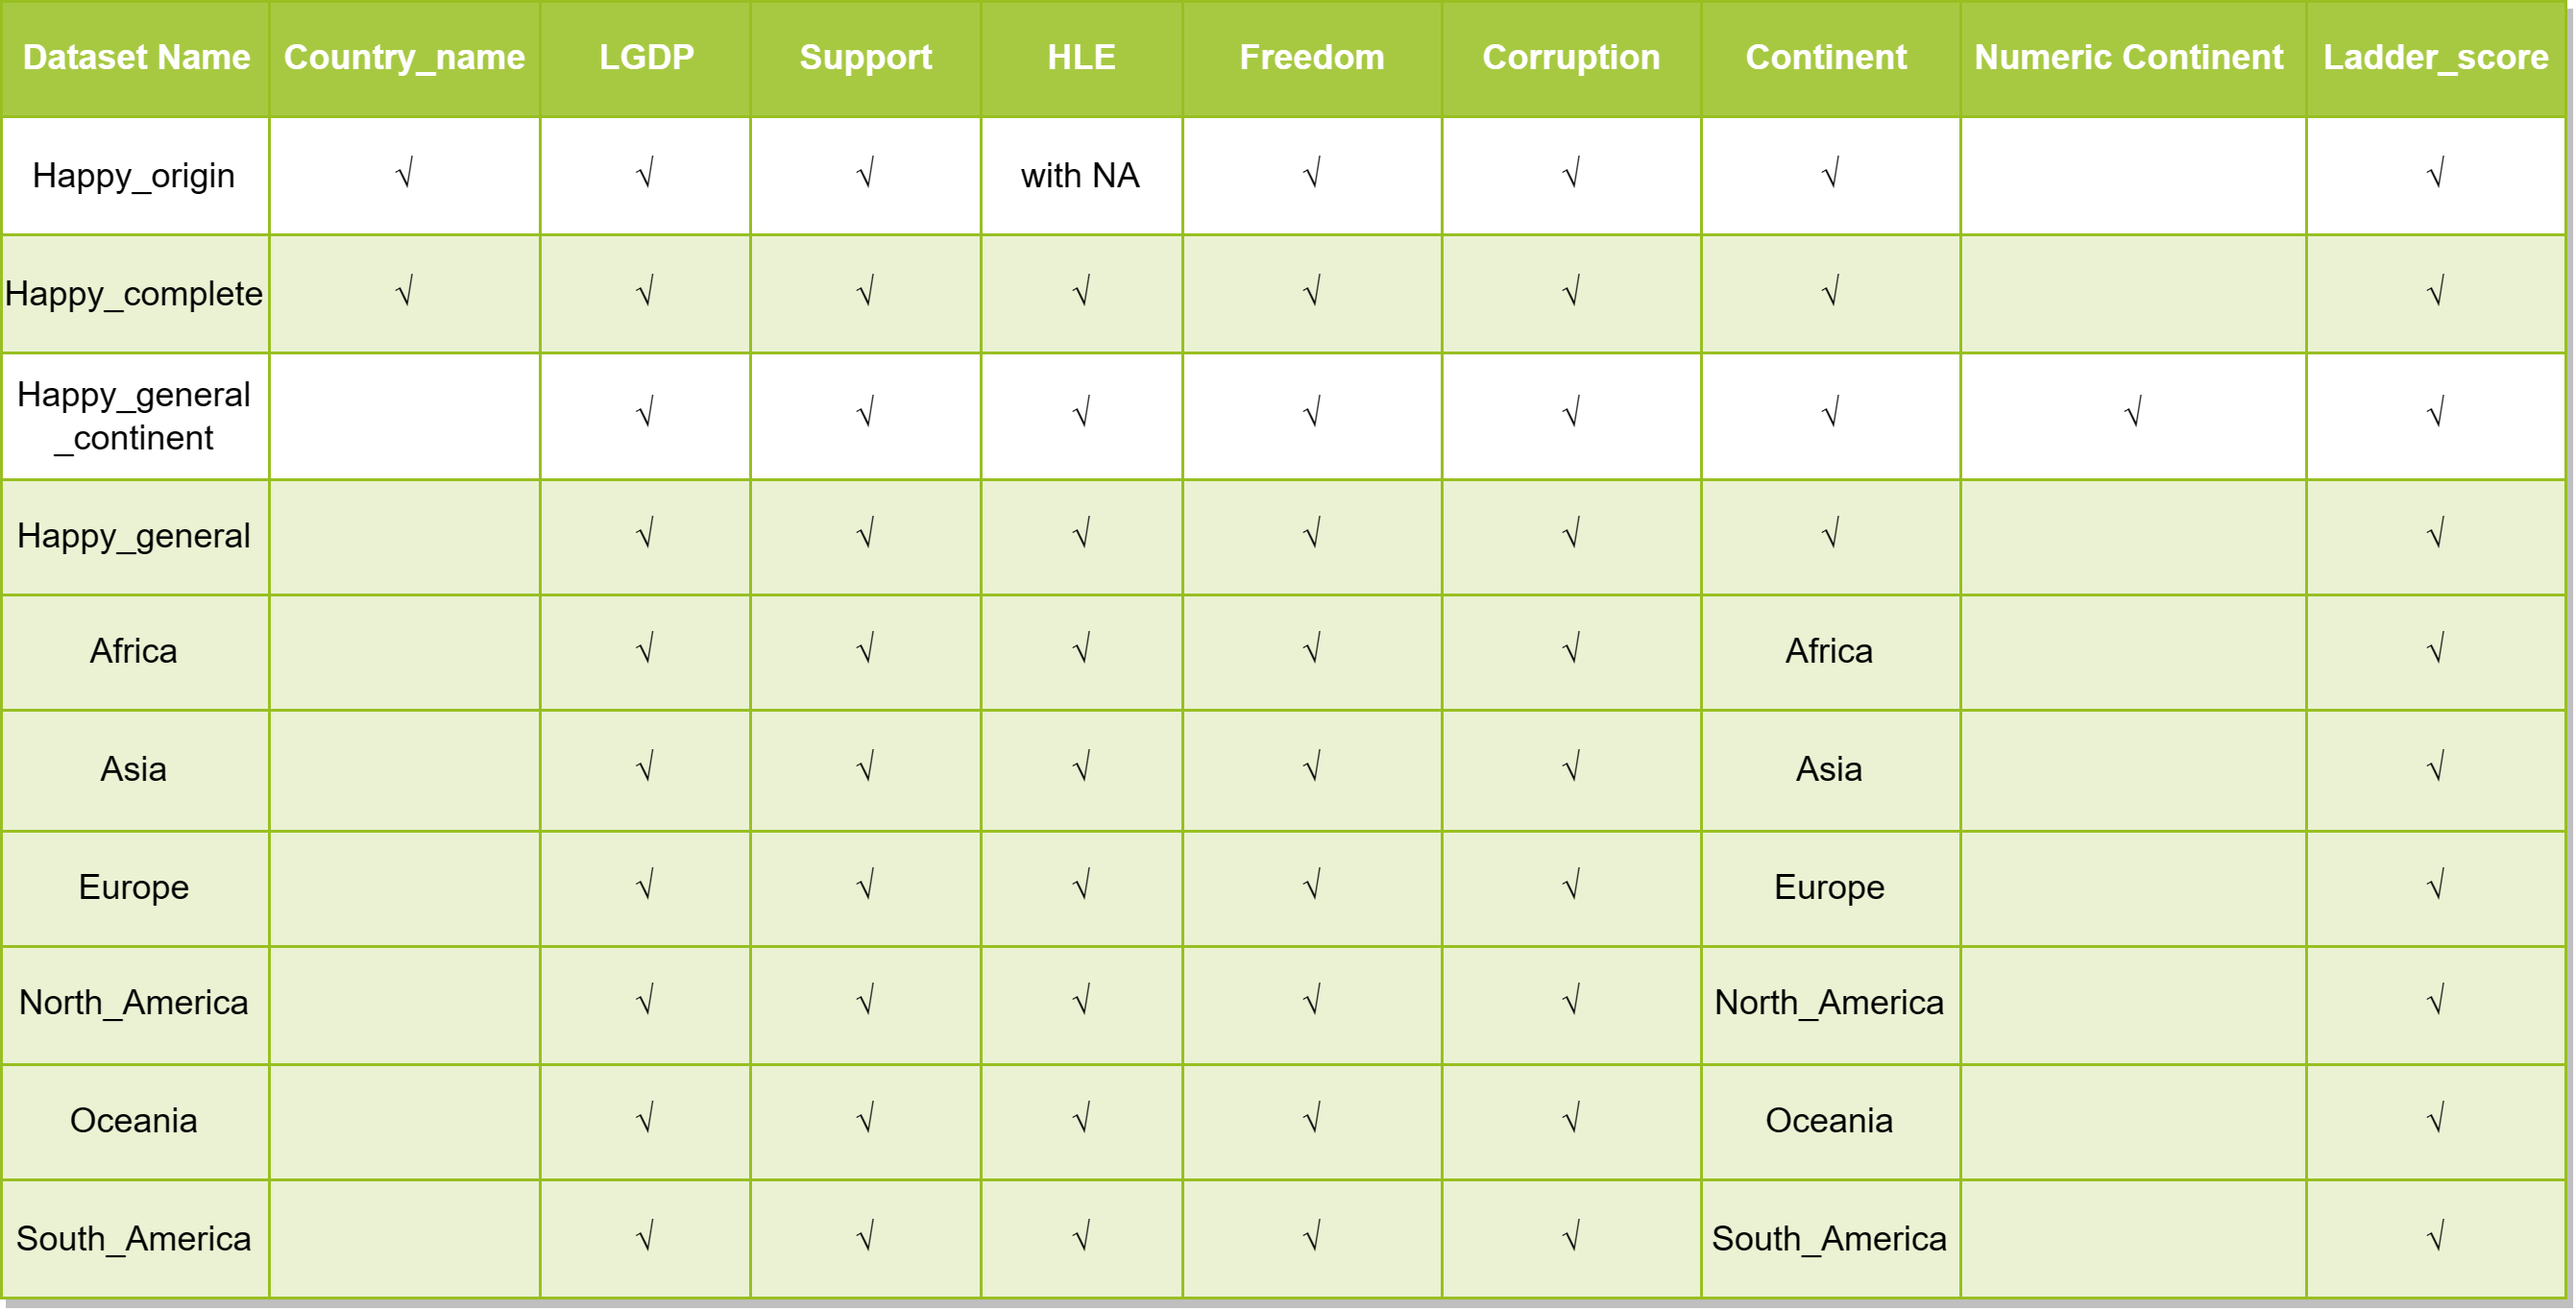
\includegraphics[width=\textwidth]{img/Dataset We have.png}
  \end{figure}
\end{frame}
% 
% 
% 
% 
% 
\begin{frame}
  \frametitle{Constructing the Model -- Bring dataset to MLR model}
  \begin{figure}
    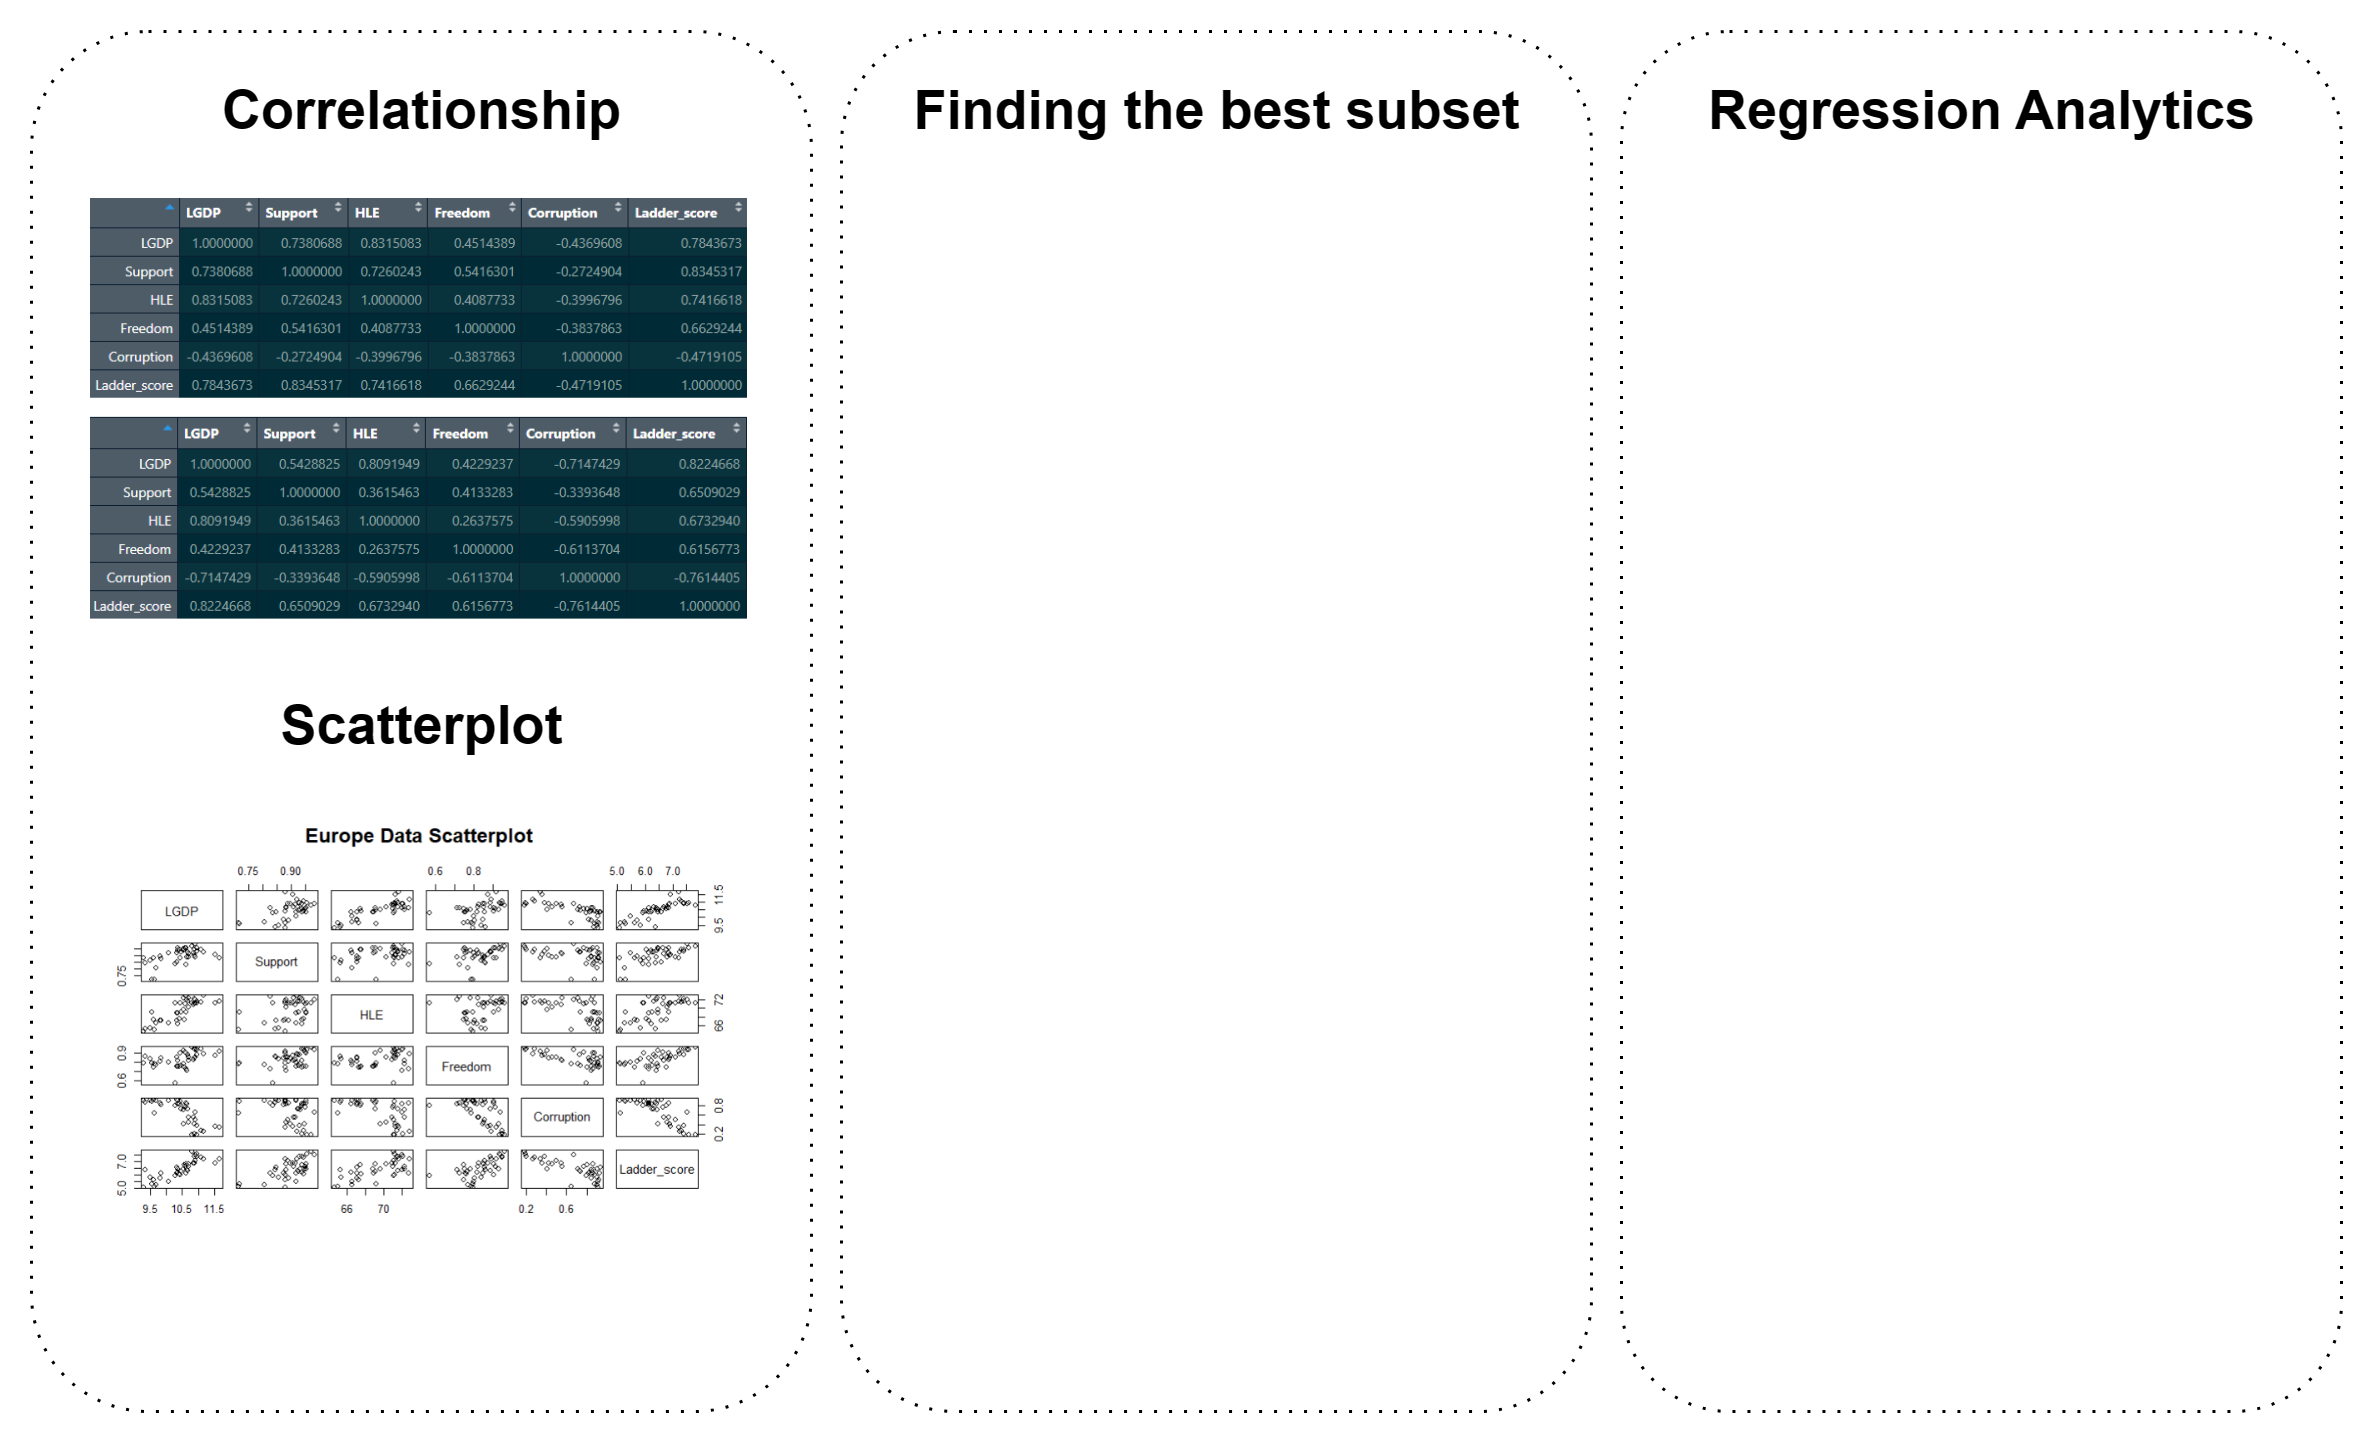
\includegraphics[width=\textwidth]{img/UsingMLR.png}
  \end{figure}
\end{frame}
% 
% 
% 
% 
% 
% 
% 
% 
% 
% 
\section{Conclusions and Analysis}
% 
% 
% 
% 
\subsection{Results and Analysis}
% 
% 
% 
% 
\begin{frame}
  \frametitle{Model Results and Analysis}
\end{frame}
% 
% 
% 
% 
\subsection{Conclusions}
% 
% 
% 
% 
\begin{frame}
  \frametitle{Conclusions and Insights}
\end{frame}
% 
% 
% 
% 
% 
% 
% 
% 
% 
% 
% 
% 
\section{Future Work}
% 
% 
% 
% 
\begin{frame}
  \frametitle{Next Steps}
\end{frame}
% \section{Introduction}
% \subsection{Background}
% \begin{frame}
%   \frametitle{The Premier League}
%   \begin{itemize}
%     \item Premier League: Top tier of English Football League System.
%     \item 20 teams play 38 home and away matches.
%     \item Globally renowned and challenging to predict outcomes.
%   \end{itemize}

%   \textbf{Background}

%   \begin{enumerate}
%     \item Outcome predictions involve expert analysis.
%     \item Factors include team performance, player form, and tactics.
%     \item Growing data, e.g., player touches, team running stats, manager experience.
%   \end{enumerate}
% \end{frame}

% % All of the following is optional and typically not needed. 
% % 
% % 
% % 
% % 
% % ----------------------------------------------------------------------
% \section{Mathematical Modeling}
% % 
% % 
% % 
% % 
% \subsection{Method 1: Entropy Weight Method in Football Team Evaluation}
% \begin{frame}
%   \frametitle{Overview of Entropy Weight Method in Football}
%   % 
%   % 
%   % 
%   % 
%   % 
%   % 
%   \begin{enumerate}
%     \item Introduction
%           \begin{itemize}
%             \item The Entropy Weight Method is a powerful analytical technique used in football team evaluation. It goes beyond traditional methods by considering the inherent information entropy within various performance attributes.
%           \end{itemize}
%     \item Key Characteristics
%           \begin{itemize}
%             \item Entropy: Reflects the degree of uncertainty or randomness within a dataset.
%             \item Weight Assignment: Assigns weights to attributes based on their information entropy.

%           \end{itemize}
%     \item Objective
%           \begin{itemize}
%             \item The method aims to provide a nuanced evaluation, giving higher importance to attributes that contribute more to understanding a team's performance.
%           \end{itemize}
%   \end{enumerate}


% \end{frame}
% % 
% % 
% % 
% % 
% \begin{frame}
%   \frametitle{Key Steps in Entropy Method}
%   \begin{enumerate}
%     \item \textbf{Data Collection and Attribute Selection}
%     \item \textbf{Entropy Calculation:}
%           \begin{itemize}
%             \item Utilize mathematical formulas to calculate the entropy of each selected attribute.
%             \item Entropy = $- \sum (p_i \cdot \log_2(p_i))$, where $p_i$ is the probability of each attribute value.
%           \end{itemize}

%     \item \textbf{Weight Assignment:}
%           \begin{itemize}
%             \item Assign weights to attributes based on their calculated entropy.
%             \item Attributes with higher entropy receive lower weights, and vice versa.
%             \item The sum of weights equals 1 for normalization.
%           \end{itemize}

%     \item \textbf{Outcome:}
%           \begin{itemize}
%             \item The result is a set of weights that reflect the relative importance of each attribute in evaluating a football team's performance.
%           \end{itemize}
%   \end{enumerate}
% \end{frame}
% % 
% % 
% \begin{frame}
%   \frametitle{Entropy Method in Our Model}
%   \begin{figure}
%     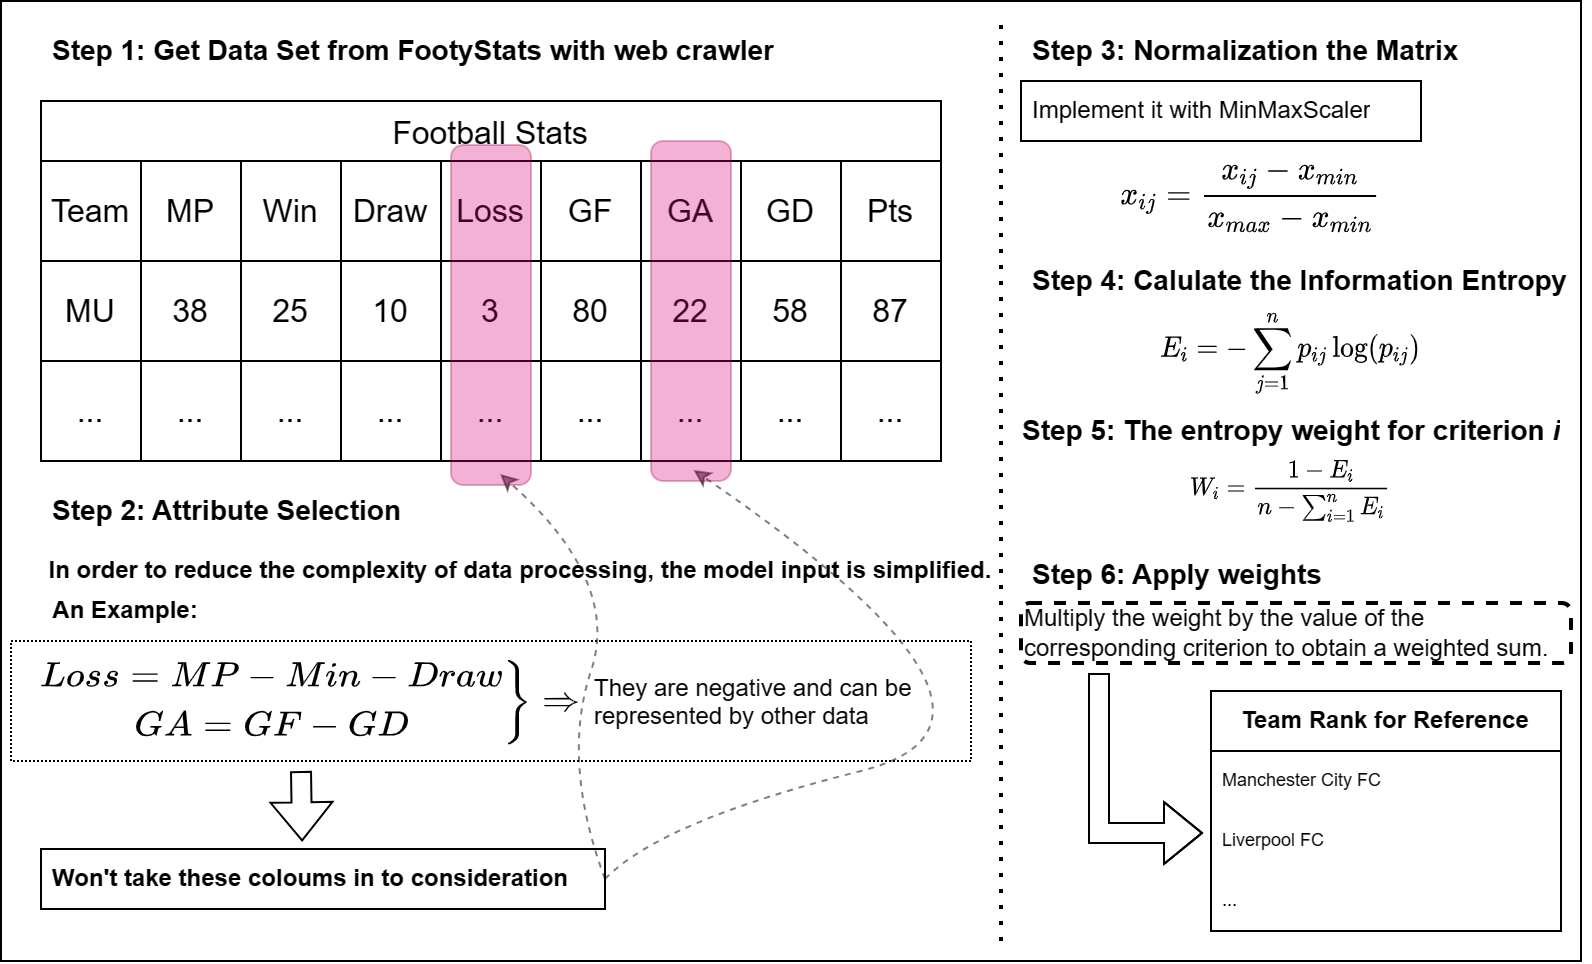
\includegraphics[width=\textwidth]{img/entropy_method_flowchart.png}
%   \end{figure}
%   % 
%   % 
% \end{frame}
% % 
% % 
% % 
% % 
% % 
% %  
% % 
% % 
% % 
% % 
% % 
% % 
% % 
% % 
% \subsection{Method 2: Linear Transformation and Gradient Ascend}
% \begin{frame}
%   \frametitle{Linear Transformation and Gradient Ascend}
%   \begin{enumerate}
%     \item Linear transformation involves transforming input variables into a new space where they are more linear and easier to model
%     \item Our model will be taking in 5-dimension vector and transforming it to a 1-dimension vector $$ F_v: \mathbb{R}^{5} \Rightarrow \mathbb{R} $$
%     \item The vector v basically consists of the following variables:
%           \begin{itemize}
%             \item The number of games won by a team in $n^{th}$ week, $v_1$
%             \item The number of games lost by a team in $n^{th}$ week, $v_2$
%             \item The number of games drawn by a team in $n^{th}$ week, $v_3$
%             \item The goal difference (goals scored - goals conceded) of a team in $n^{th}$ week, $v_4$
%             \item The number of points scored by a team in $n^{th}$ week, $v_5$
%           \end{itemize}
%   \end{enumerate}
% \end{frame}
% % 
% % 
% % 
% % 
% % 
% % 
% % 
% % 
% \begin{frame}
%   \frametitle{Linear Transformation and Gradient Ascend}
%   \begin{itemize}
%     \item The linear transformation will transform the 5-dimensional vector into a one-dimensional vector which is the total number of points in the final week $F(v)$
%     \item To calculate we will use the following formula: $$ F(v)=wv+b $$
%     \item $w$ is a 5-dimensional vector, weights of each variable in vector v
%     \item $b$ is the scalar bias - systematic error

%   \end{itemize}
% \end{frame}
% % 
% % 
% % 
% % 
% % 
% \begin{frame}
%   \frametitle{Using Gradient Ascend}
%   \begin{itemize}
%     \item To calculate w and b, we will use gradient ascend on historical data.
%     \item Normalize $v$ and $F(v)$ by centering and standardizing it.
%     \item Use normalized data and take out predicted points using any initial value of weight.
%     \item See the error by finding the difference between normalized $F(v)$ and predicted $F(v)$
%     \item Find the gradient of the weight using the formula - transposed-v.error
%     \item Find the gradient of scalar bias using the formula - sum of all elements in error vector
%     \item Then to find the updated gradient the following formula is:
%     $$ w = w + a*w_{gradient}, \ b = b + a*b_{gradient} $$
%     \item Then denormalize w and b to find the actual values

%   \end{itemize}
% \end{frame}
% % 
% % 
% % 
% % 
% \section{Result Analysis}
% \subsection{Grabbing Data from Web}
% \begin{frame}
%   \frametitle{Grabbing Data from Web}
%   \begin{figure}
%     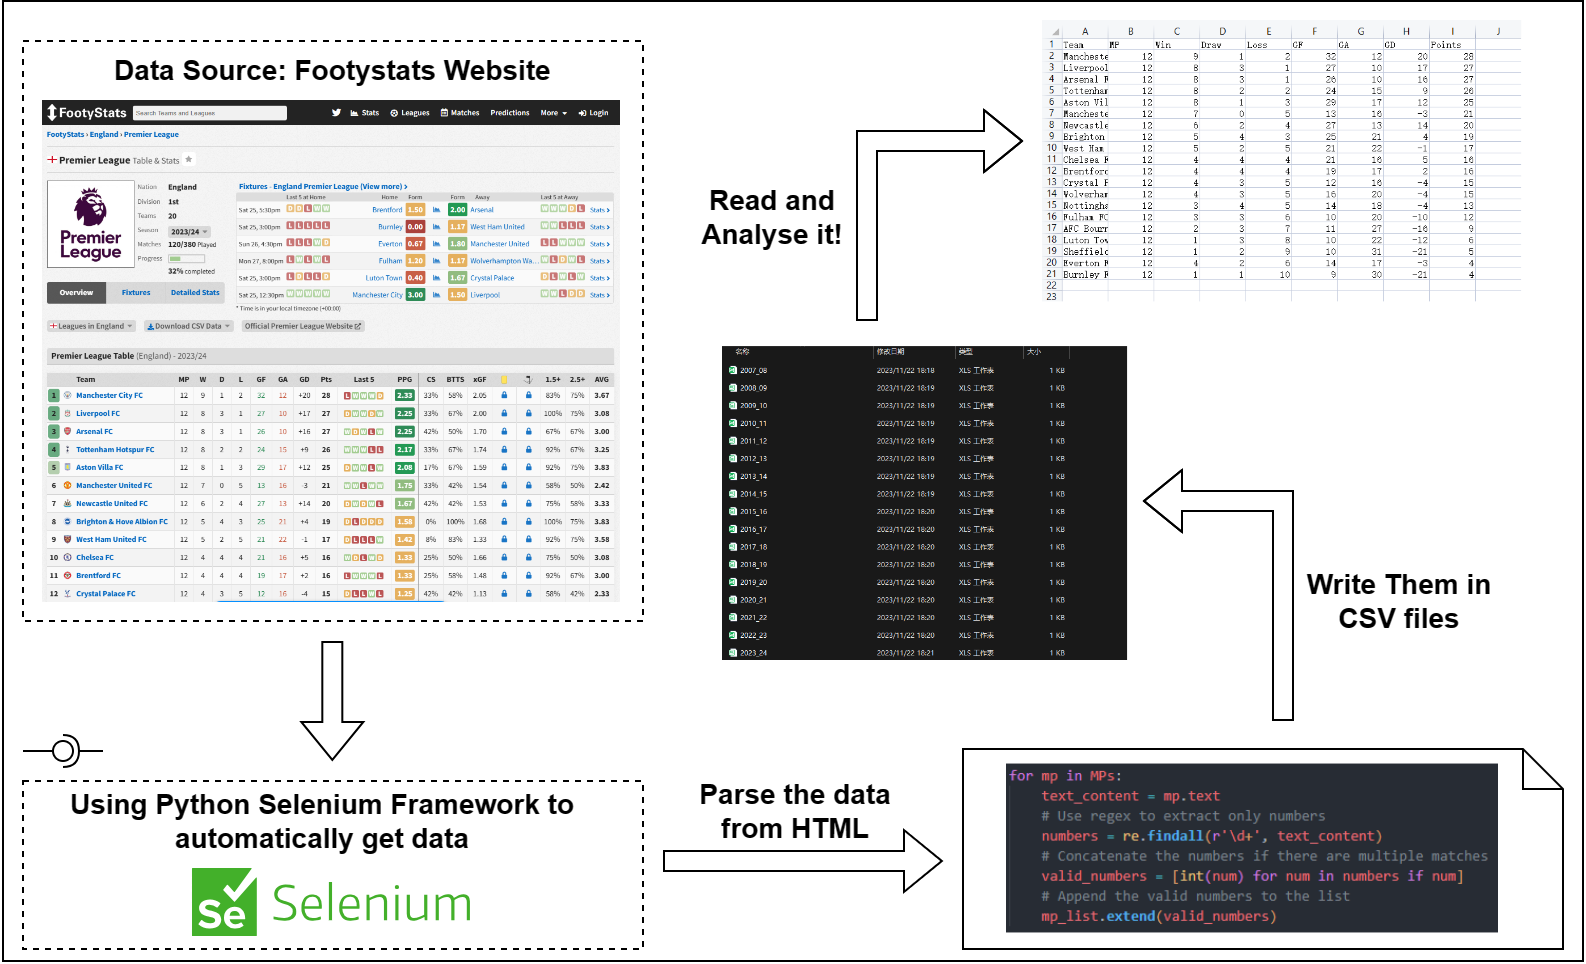
\includegraphics[width=\textwidth]{img/DataGrab.png}
%   \end{figure}
% \end{frame}
% \subsection{Evaluating the Teams's Tier}
% \begin{frame}
%   \frametitle{Evaluating the Teams's Tier with Entropy Method}
%   \begin{figure}
%     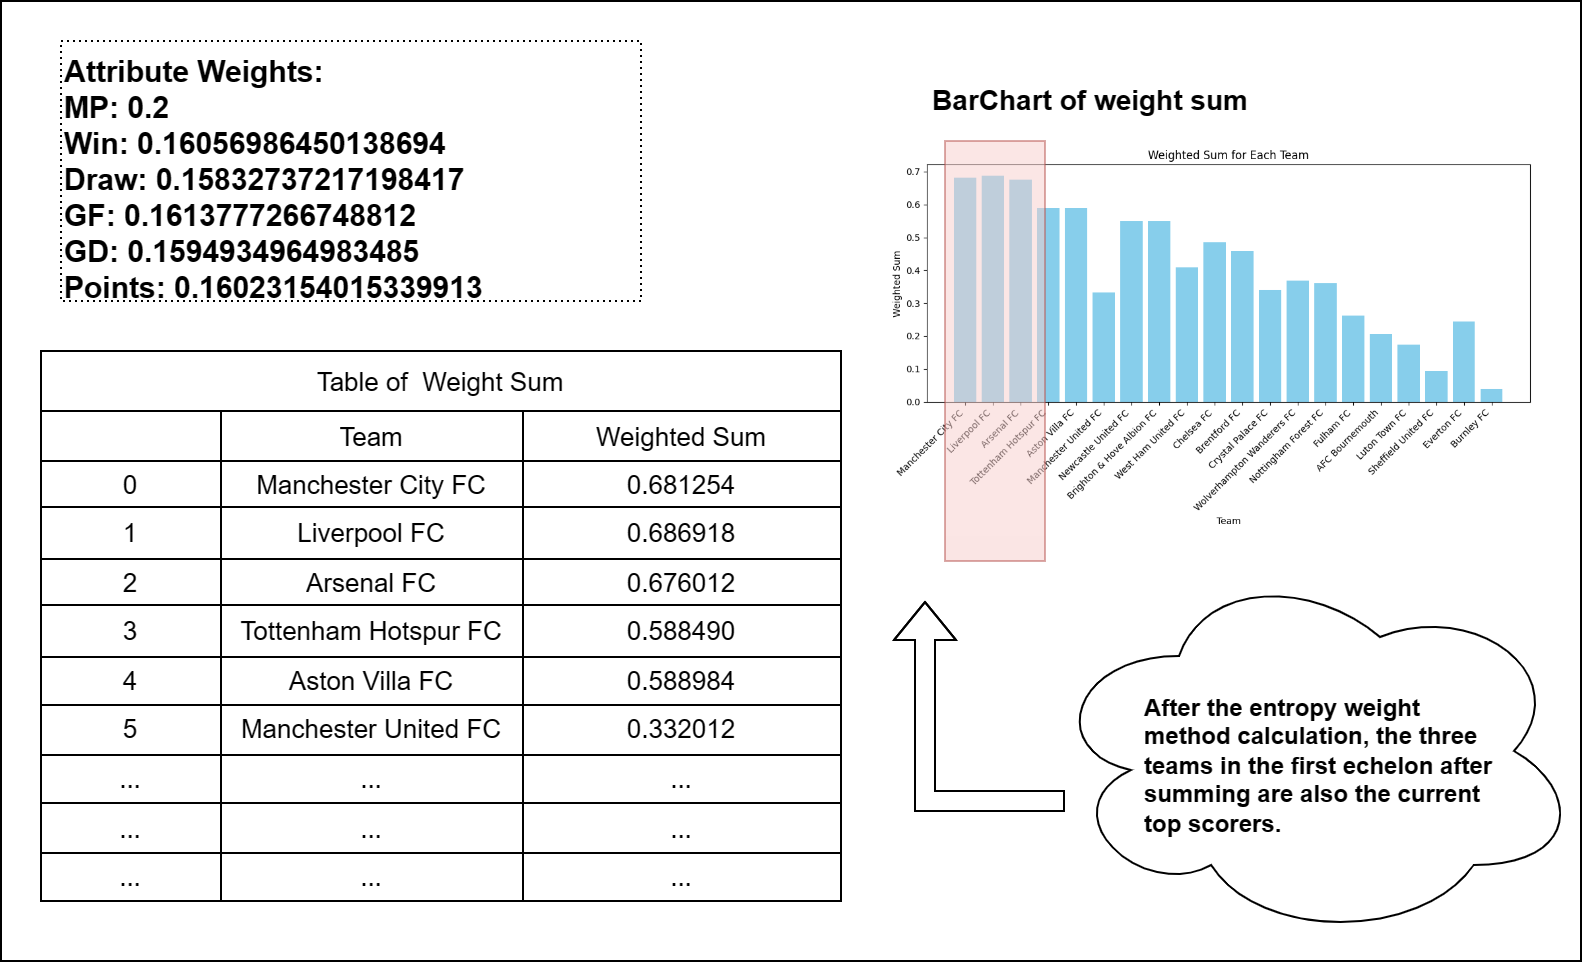
\includegraphics[width=\textwidth]{img/Entropy_output.png}
%   \end{figure}
% \end{frame}
% % 
% % 
% % 
% % Prediction of 2023/24's final point
% % 
% % 
% % 
% \subsection{Prediction of 2023/24's winner point}
% \begin{frame}
%   \frametitle{Prediction of 2023/24's winner point}
%   \begin{figure}
%     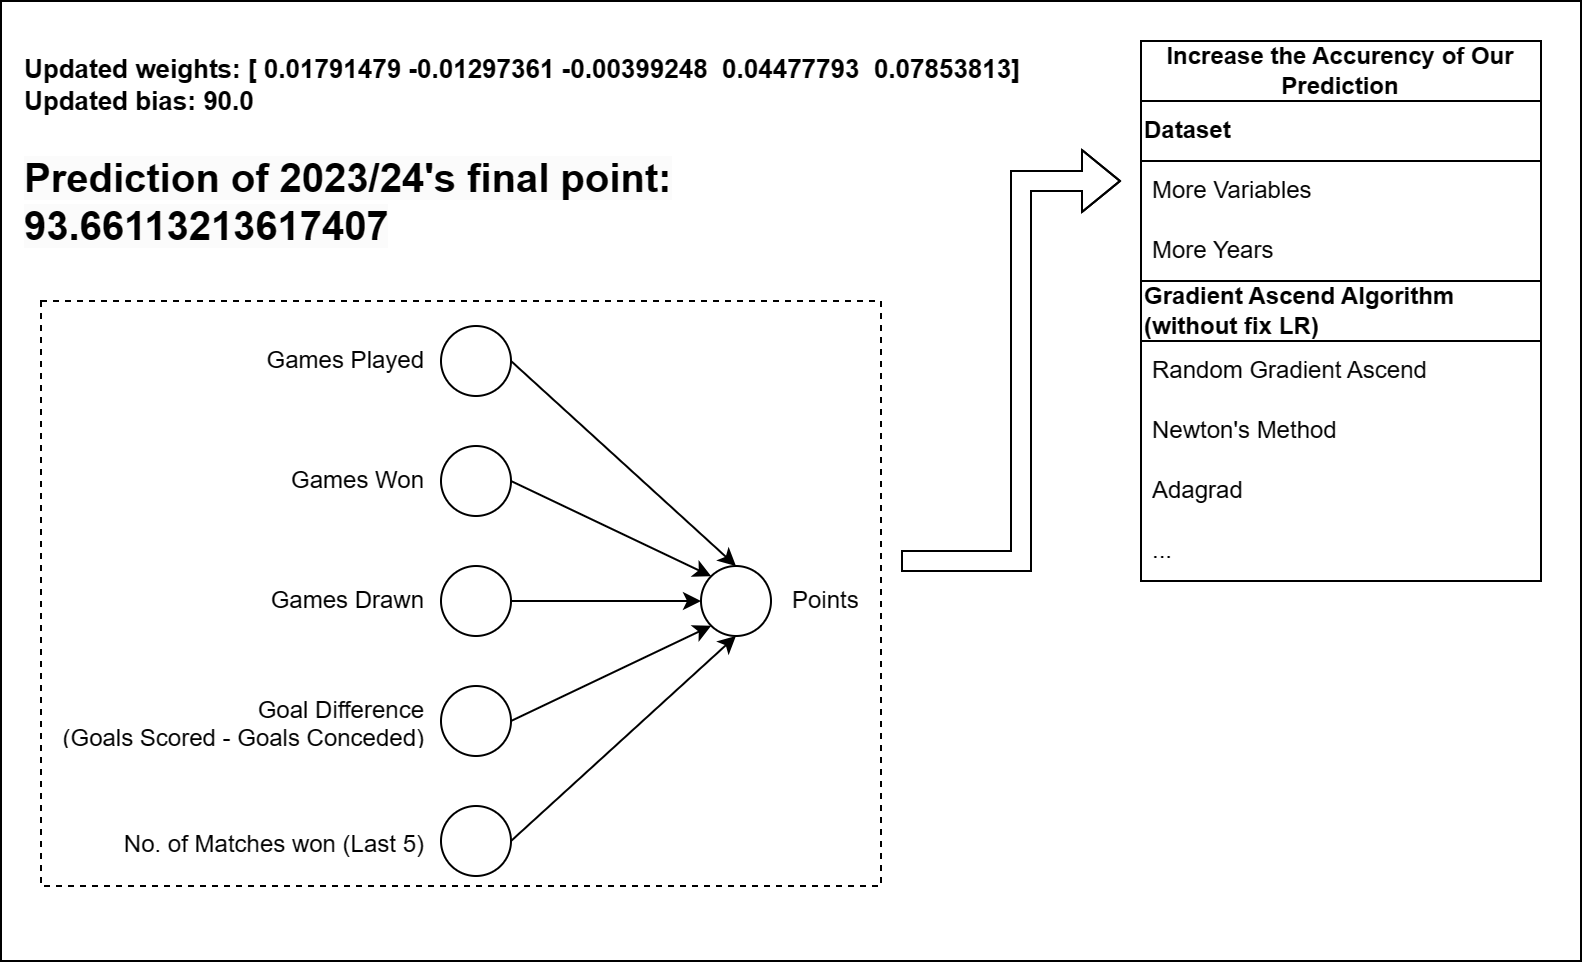
\includegraphics[width=\textwidth]{img/prediction_current_year.png}
%   \end{figure}
% \end{frame}
% % 
% % 
% % 
% % 
% % 
% % 
% % 
% % 
% \section{Future Work}
% \subsection{Our plans, our limitations and how these models could improve}
% \begin{frame}
%   \frametitle{Future plans}
%   \begin{itemize}
%     \item Once our models are all complete, we will compare them with respect to efficiency and accuracy in predicting the winning team with this year's data as input. We could make use of Mallows' Cp and BIC statistic to establish which model has the best predictive performance.
%     \item We will then critically analyse the most successful model and input a test dataset from earlier years to ensure we have not overfitted to our training dataset.
%     \item To improve this model, it would be wise to consider variables other than the teams' performance and establish whether they are confounding and extraneous; for example, the about of money invested in each team.
%   \end{itemize}
% \end{frame}
% 
% 
% 
% 
% 
% 
% 

% \begin{frame}
%   \frametitle{What is this model useful for}
%   \begin{enumerate}
%     \item Once the most significant variables have been established, a researcher could potentially use the model to advise  a team's manager of where best to focus their efforts, or indeed they could consult with a bookie to help them predict the odds of the game.
%     \item Of course, this model overlooks the human element of the game. Factors that a manager might be aware of such as player motivation, injuries, and team dynamics can have a significant impact on the outcome of a game, but they are challenging to factor into our model.
%     \item Ultimately though, it is impossible to control for every variable and, even if we did the result could surprise us. But this model is beneficial in finding which variables give the teams the best chance of success.
%   \end{enumerate}
% \end{frame}
% 
% 
% 
% 
% 
% 
% 
% 
\end{document}
